\documentclass[]{article}
\usepackage{lmodern}
\usepackage{amssymb,amsmath}
\usepackage{ifxetex,ifluatex}
\usepackage{fixltx2e} % provides \textsubscript
\ifnum 0\ifxetex 1\fi\ifluatex 1\fi=0 % if pdftex
  \usepackage[T1]{fontenc}
  \usepackage[utf8]{inputenc}
\else % if luatex or xelatex
  \ifxetex
    \usepackage{mathspec}
  \else
    \usepackage{fontspec}
  \fi
  \defaultfontfeatures{Ligatures=TeX,Scale=MatchLowercase}
\fi
% use upquote if available, for straight quotes in verbatim environments
\IfFileExists{upquote.sty}{\usepackage{upquote}}{}
% use microtype if available
\IfFileExists{microtype.sty}{%
\usepackage[]{microtype}
\UseMicrotypeSet[protrusion]{basicmath} % disable protrusion for tt fonts
}{}
\PassOptionsToPackage{hyphens}{url} % url is loaded by hyperref
\usepackage[unicode=true]{hyperref}
\hypersetup{
            pdftitle={Using k-Means to Cluster Tweets},
            pdfauthor={Jana Osea and Evan Quan},
            pdfborder={0 0 0},
            breaklinks=true}
\urlstyle{same}  % don't use monospace font for urls
\usepackage[margin=1in]{geometry}
\usepackage{graphicx,grffile}
\makeatletter
\def\maxwidth{\ifdim\Gin@nat@width>\linewidth\linewidth\else\Gin@nat@width\fi}
\def\maxheight{\ifdim\Gin@nat@height>\textheight\textheight\else\Gin@nat@height\fi}
\makeatother
% Scale images if necessary, so that they will not overflow the page
% margins by default, and it is still possible to overwrite the defaults
% using explicit options in \includegraphics[width, height, ...]{}
\setkeys{Gin}{width=\maxwidth,height=\maxheight,keepaspectratio}
\IfFileExists{parskip.sty}{%
\usepackage{parskip}
}{% else
\setlength{\parindent}{0pt}
\setlength{\parskip}{6pt plus 2pt minus 1pt}
}
\setlength{\emergencystretch}{3em}  % prevent overfull lines
\providecommand{\tightlist}{%
  \setlength{\itemsep}{0pt}\setlength{\parskip}{0pt}}
\setcounter{secnumdepth}{0}
% Redefines (sub)paragraphs to behave more like sections
\ifx\paragraph\undefined\else
\let\oldparagraph\paragraph
\renewcommand{\paragraph}[1]{\oldparagraph{#1}\mbox{}}
\fi
\ifx\subparagraph\undefined\else
\let\oldsubparagraph\subparagraph
\renewcommand{\subparagraph}[1]{\oldsubparagraph{#1}\mbox{}}
\fi

% set default figure placement to htbp
\makeatletter
\def\fps@figure{htbp}
\makeatother

\usepackage{booktabs}
\usepackage{longtable}
\usepackage{array}
\usepackage{multirow}
\usepackage{wrapfig}
\usepackage{float}
\usepackage{colortbl}
\usepackage{pdflscape}
\usepackage{tabu}
\usepackage{threeparttable}
\usepackage{threeparttablex}
\usepackage[normalem]{ulem}
\usepackage{makecell}
\usepackage{xcolor}

\title{Using k-Means to Cluster Tweets}
\author{Jana Osea and Evan Quan}
\date{November 24, 2020}

\begin{document}
\maketitle

\subsection{Dataset Previews}\label{dataset-previews}

We will use three datasets scraped from Twitter on November 22, 2020
using \(n=100\) tweets.

\begin{enumerate}
\def\labelenumi{\arabic{enumi}.}
\item
  Raw Scraped Dataset

  \begin{table}[H]
  \centering
  \begin{tabular}[t]{l|l|r|l|l|l|r|r|r|l|l|r|l|l|l|l|r|r|l|r}
  \hline
  text & favorited & favoriteCount & replyToSN & created & truncated & replyToSID & id & replyToUID & statusSource & screenName & retweetCount & isRetweet & retweeted & longitude & latitude & followers & total\_tweets & location & score\\
  \hline
  RT @yyynagoham: Idk why the student loan ppl emailed me today about my payments starting back up In January lol they better reach out to Jo… & FALSE & 0 & NA & 2020-11-24 6:38 & FALSE & NA & 1.33112e+18 & NA & <a href="http://twitter.com/download/iphone" rel="nofollow">Twitter for iPhone</a> & the\_GoldenOreo & 13 & TRUE & FALSE & NA & NA & 583 & 126645 & Angeles Los, Ca<U+2600><U+FE0F> & 0\\
  \hline
  RT @bocxtop: what is joe biden’s plan to stop the sun from disappearing at 5pm & FALSE & 0 & NA & 2020-11-24 6:38 & FALSE & NA & 1.33112e+18 & NA & <a href="http://twitter.com/download/iphone" rel="nofollow">Twitter for iPhone</a> & badwisglory & 26215 & TRUE & FALSE & NA & NA & 120 & 12455 &  & 3\\
  \hline
  Top story: President-Elect Joe Biden: Official Transition Website https://t.co/ROq6Q6aw5r, see more https://t.co/JXkTW2SeqS & FALSE & 0 & NA & 2020-11-24 6:38 & FALSE & NA & 1.33112e+18 & NA & <a href="https://www.tweetedtimes.com" rel="nofollow">The Tweeted Times</a> & sds\_labs & 0 & FALSE & FALSE & NA & NA & 2642 & 71825 & EU & 7\\
  \hline
  \end{tabular}
  \end{table}
\item
  Processed Scaled Tweets

  \begin{table}[H]
  \centering
  \begin{tabular}[t]{r|r|r|r|r|r}
  \hline
  total\_tweets & followers & retweetCount & score & isRetweet & created\\
  \hline
  0.7391004 & -0.3435185 & -0.3547303 & -0.8500081 & 0.7462406 & 1.683726\\
  \hline
  -0.4247244 & -0.4671545 & 5.0821002 & 0.5209727 & 0.7462406 & 1.480377\\
  \hline
  0.1803748 & 0.2063012 & -0.3574277 & 2.3489470 & -1.3266499 & 1.480377\\
  \hline
  \end{tabular}
  \end{table}
\item
  Top 10 Common Words

  \begin{table}[H]
  \centering
  \begin{tabular}[t]{l|r}
  \hline
  word & n\\
  \hline
  joe & 41\\
  \hline
  transition & 26\\
  \hline
  president & 25\\
  \hline
  \end{tabular}
  \end{table}
\end{enumerate}

\subsection{k-Means Clustering}\label{k-means-clustering}

We plotted the cluster plots with \(k=2,3,4,5\) clusters
correspondingly.
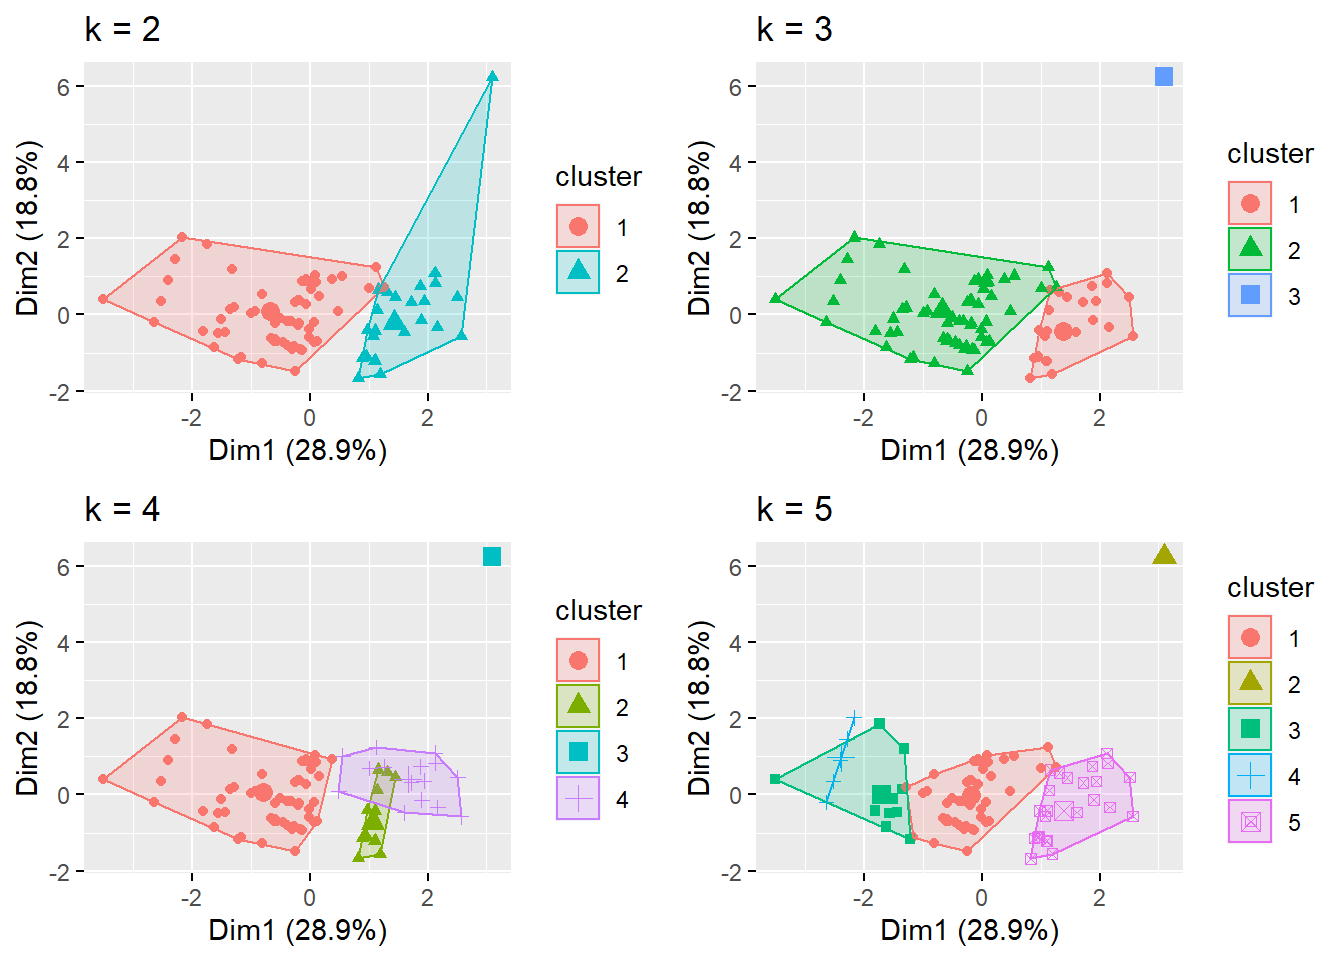
\includegraphics{output_files/figure-latex/unnamed-chunk-5-1.pdf}

We choose \(k=3\) as our chosen number of clusters and we will now
analyze.

\subsection{\texorpdfstring{\(k=3\) Means Clustering
Analysis}{k=3 Means Clustering Analysis}}\label{k3-means-clustering-analysis}

\paragraph{Variation Between, Within and
Total}\label{variation-between-within-and-total}

\begin{table}[H]
\centering
\begin{tabular}[t]{l|r}
\hline
Sum.of.Squares & Values\\
\hline
Between & 204.4527\\
\hline
Total & 594.0000\\
\hline
\end{tabular}
\end{table}

\begin{table}[H]
\centering
\begin{tabular}[t]{r|r}
\hline
Cluster & Within.Sum.of.Squares\\
\hline
1 & 181.35826\\
\hline
2 & 98.95181\\
\hline
3 & 109.23726\\
\hline
\end{tabular}
\end{table}

\paragraph{1. Common Words}\label{common-words}

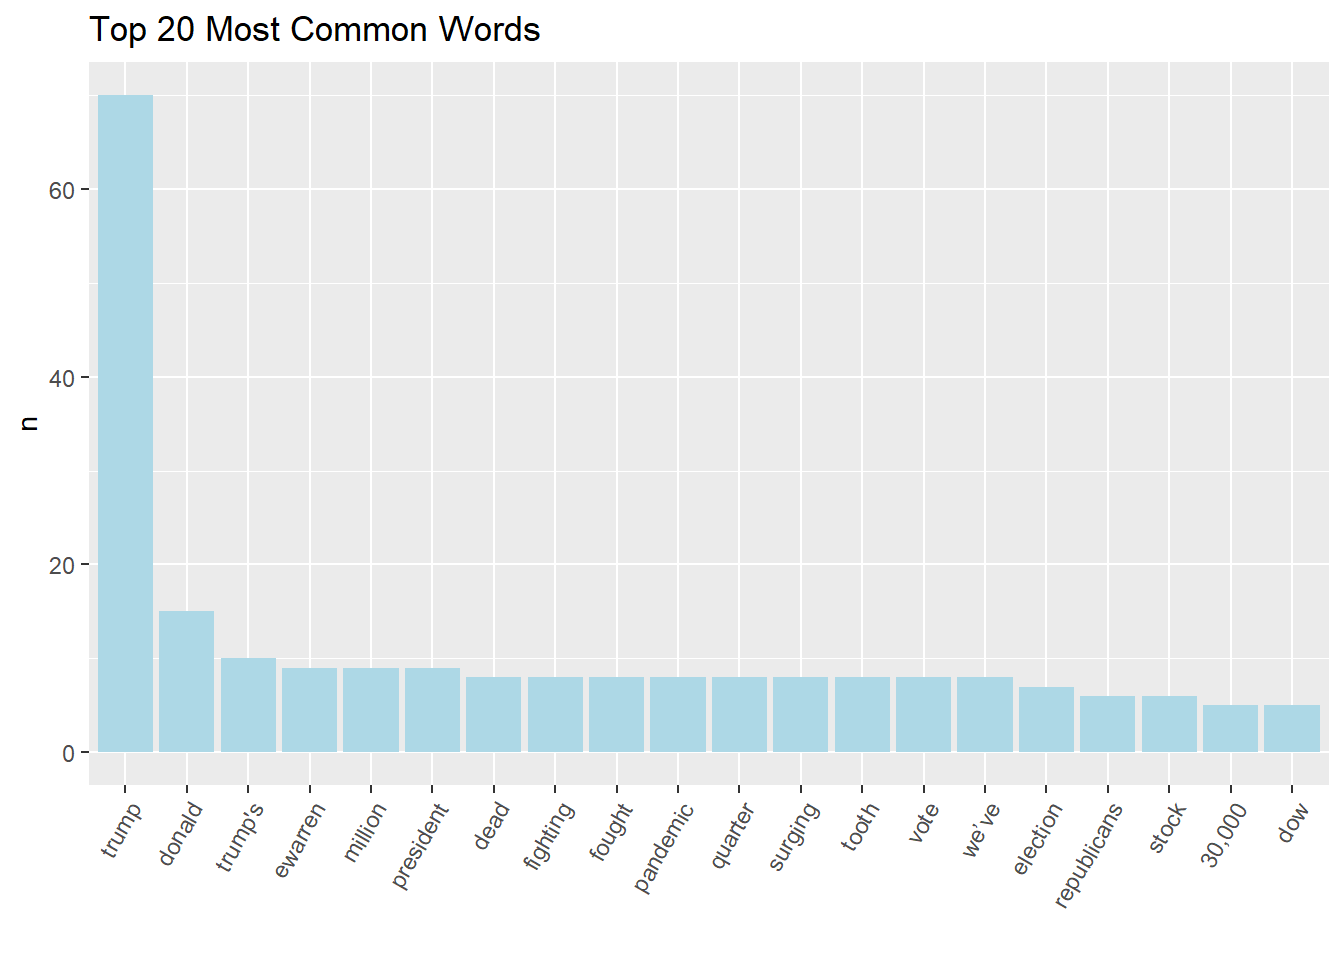
\includegraphics{output_files/figure-latex/unnamed-chunk-7-1.pdf}

\paragraph{2. Hot Word Scores}\label{hot-word-scores}

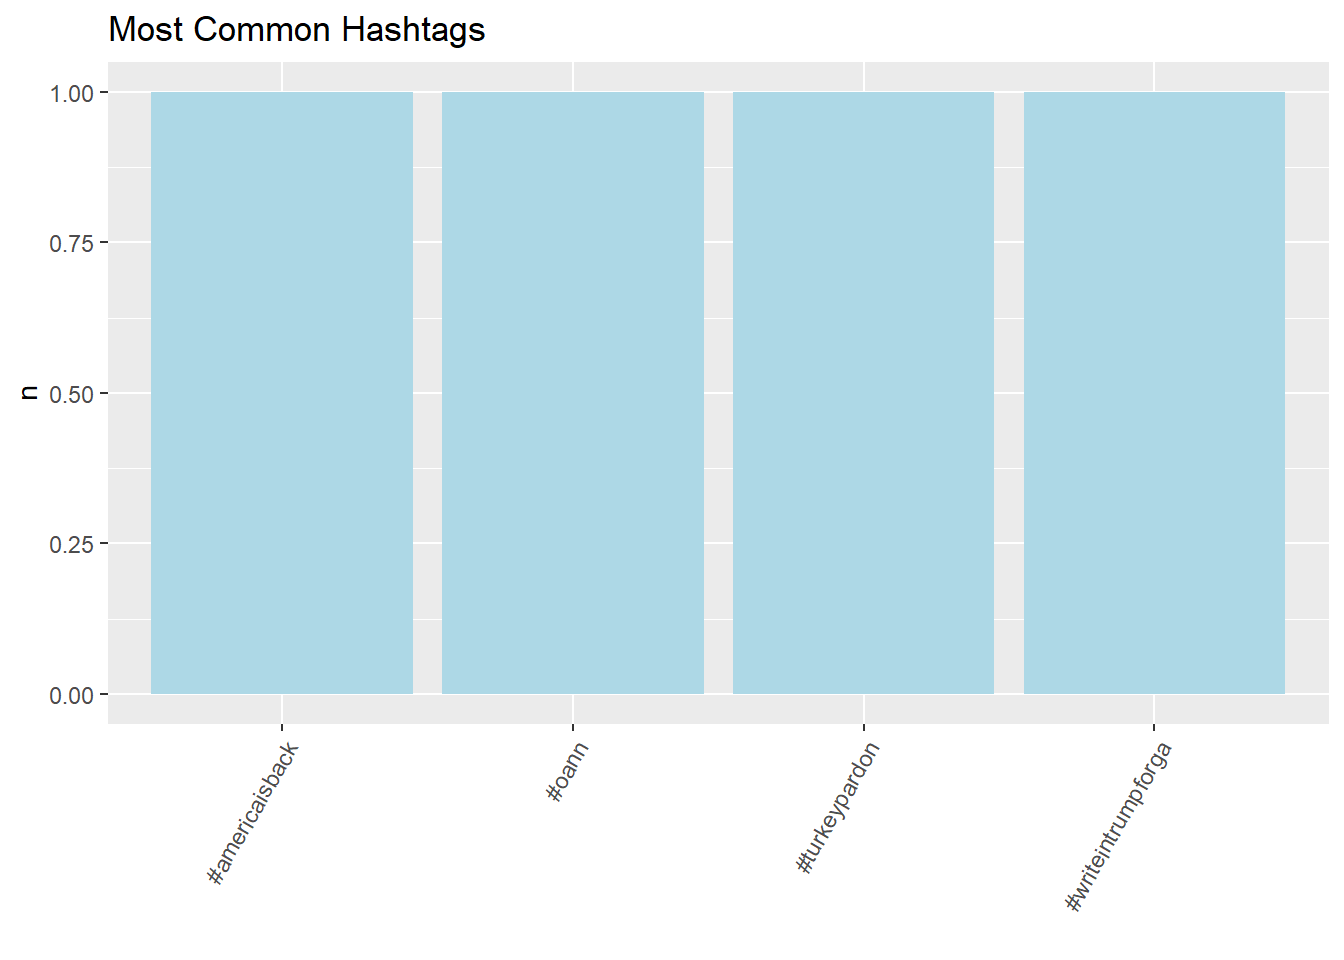
\includegraphics{output_files/figure-latex/unnamed-chunk-8-1.pdf}

\paragraph{3. Compare Characteristics of Each
Cluster}\label{compare-characteristics-of-each-cluster}

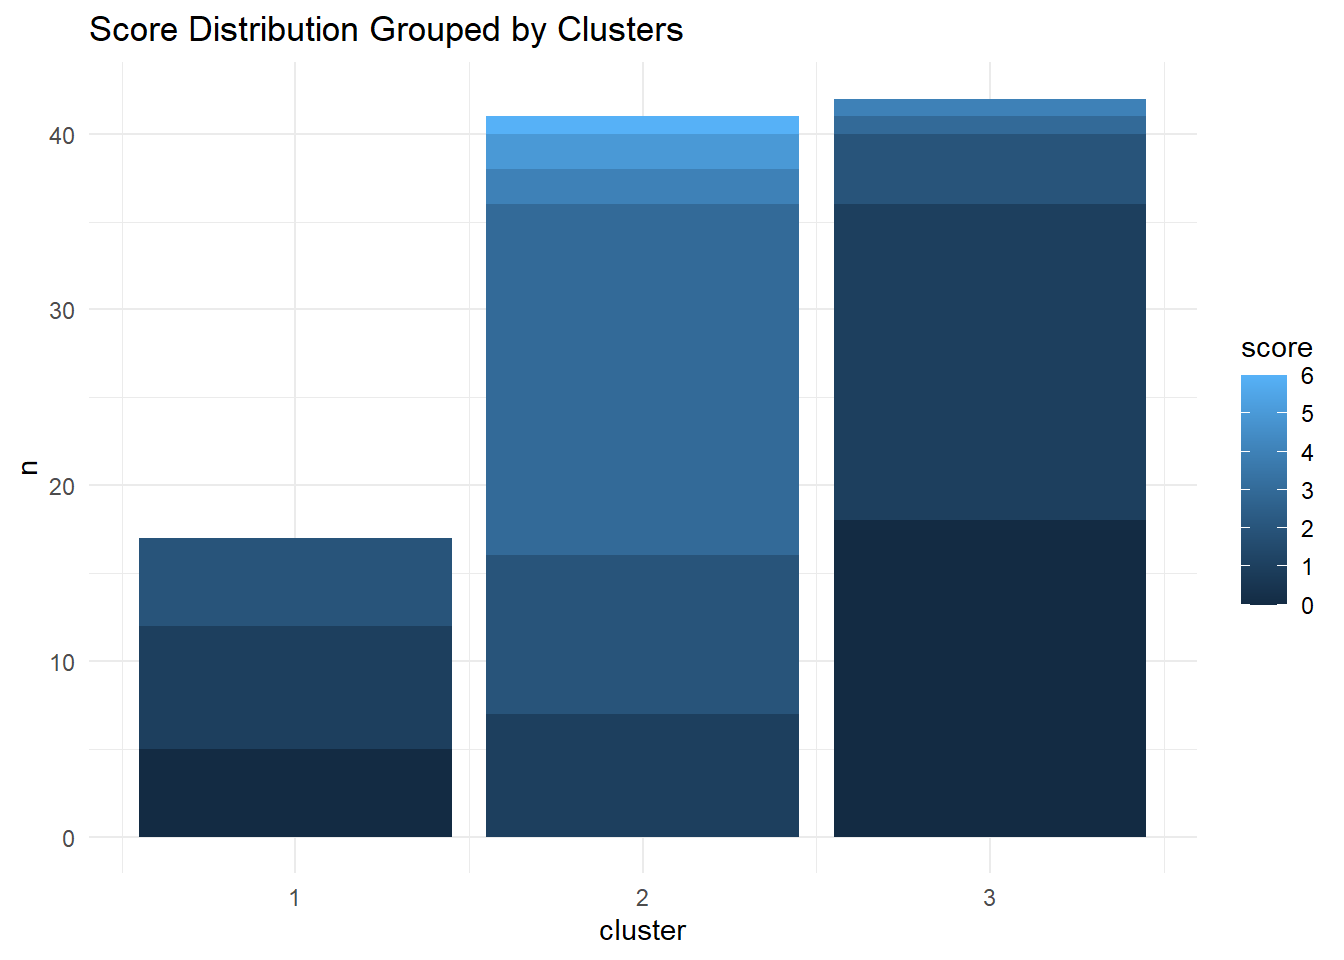
\includegraphics{output_files/figure-latex/unnamed-chunk-9-1.pdf}
\includegraphics{output_files/figure-latex/unnamed-chunk-9-2.pdf}
\includegraphics{output_files/figure-latex/unnamed-chunk-9-3.pdf}
\includegraphics{output_files/figure-latex/unnamed-chunk-9-4.pdf}

\paragraph{4. Top 5 Nearest Tweets to Each Centroid
Cluster}\label{top-5-nearest-tweets-to-each-centroid-cluster}

\begin{verbatim}
## Adding missing grouping variables: `cluster`
\end{verbatim}

\begin{table}[H]
\centering
\begin{tabular}[t]{r|l|r|r|l|r}
\hline
cluster & screenName & followers & total\_tweets & location & score\\
\hline
1 & tangledupinlust & 98 & 2519 & Emmitsburg, MD & 4\\
\hline
1 & zaxoguda & 6350 & 63273 & Nairobi & 2\\
\hline
1 & Butrphli & 403 & 18552 & Earth & 1\\
\hline
1 & slimwhit69 & 192 & 42379 & Fort Wayne, IN & 1\\
\hline
1 & dariasito & 67 & 713 &  & 2\\
\hline
2 & ae4ca & 3009 & 369339 & Atlanta, GA & 3\\
\hline
2 & epeterd916 & 1772 & 313330 &  & 0\\
\hline
2 & libbyliberalnyc & 5030 & 467130 & New York, USA & 0\\
\hline
2 & 99ermikeb & 13288 & 158529 & Nidaveillire & 1\\
\hline
2 & designsbycary & 14278 & 11395 & The Colony, TX & 0\\
\hline
3 & TheObservatory\_ & 7 & 1413 &  & 1\\
\hline
3 & RachDaBrat & 2249 & 141677 & Jamaica & 3\\
\hline
3 & Monet4 & 1 & 24 & United States & 0\\
\hline
3 & jennythigpen & 296 & 8732 & Florence, AL & 0\\
\hline
3 & weranwithwolves & 859 & 11754 & Colorado, USA & 3\\
\hline
\end{tabular}
\end{table}

\end{document}
